\section{Повторение основных моделей. Автоматическое дифференцирование.}

\subsection{Многослойный перцептрон}
\begin{figure}[h!t]\center
\subfloat{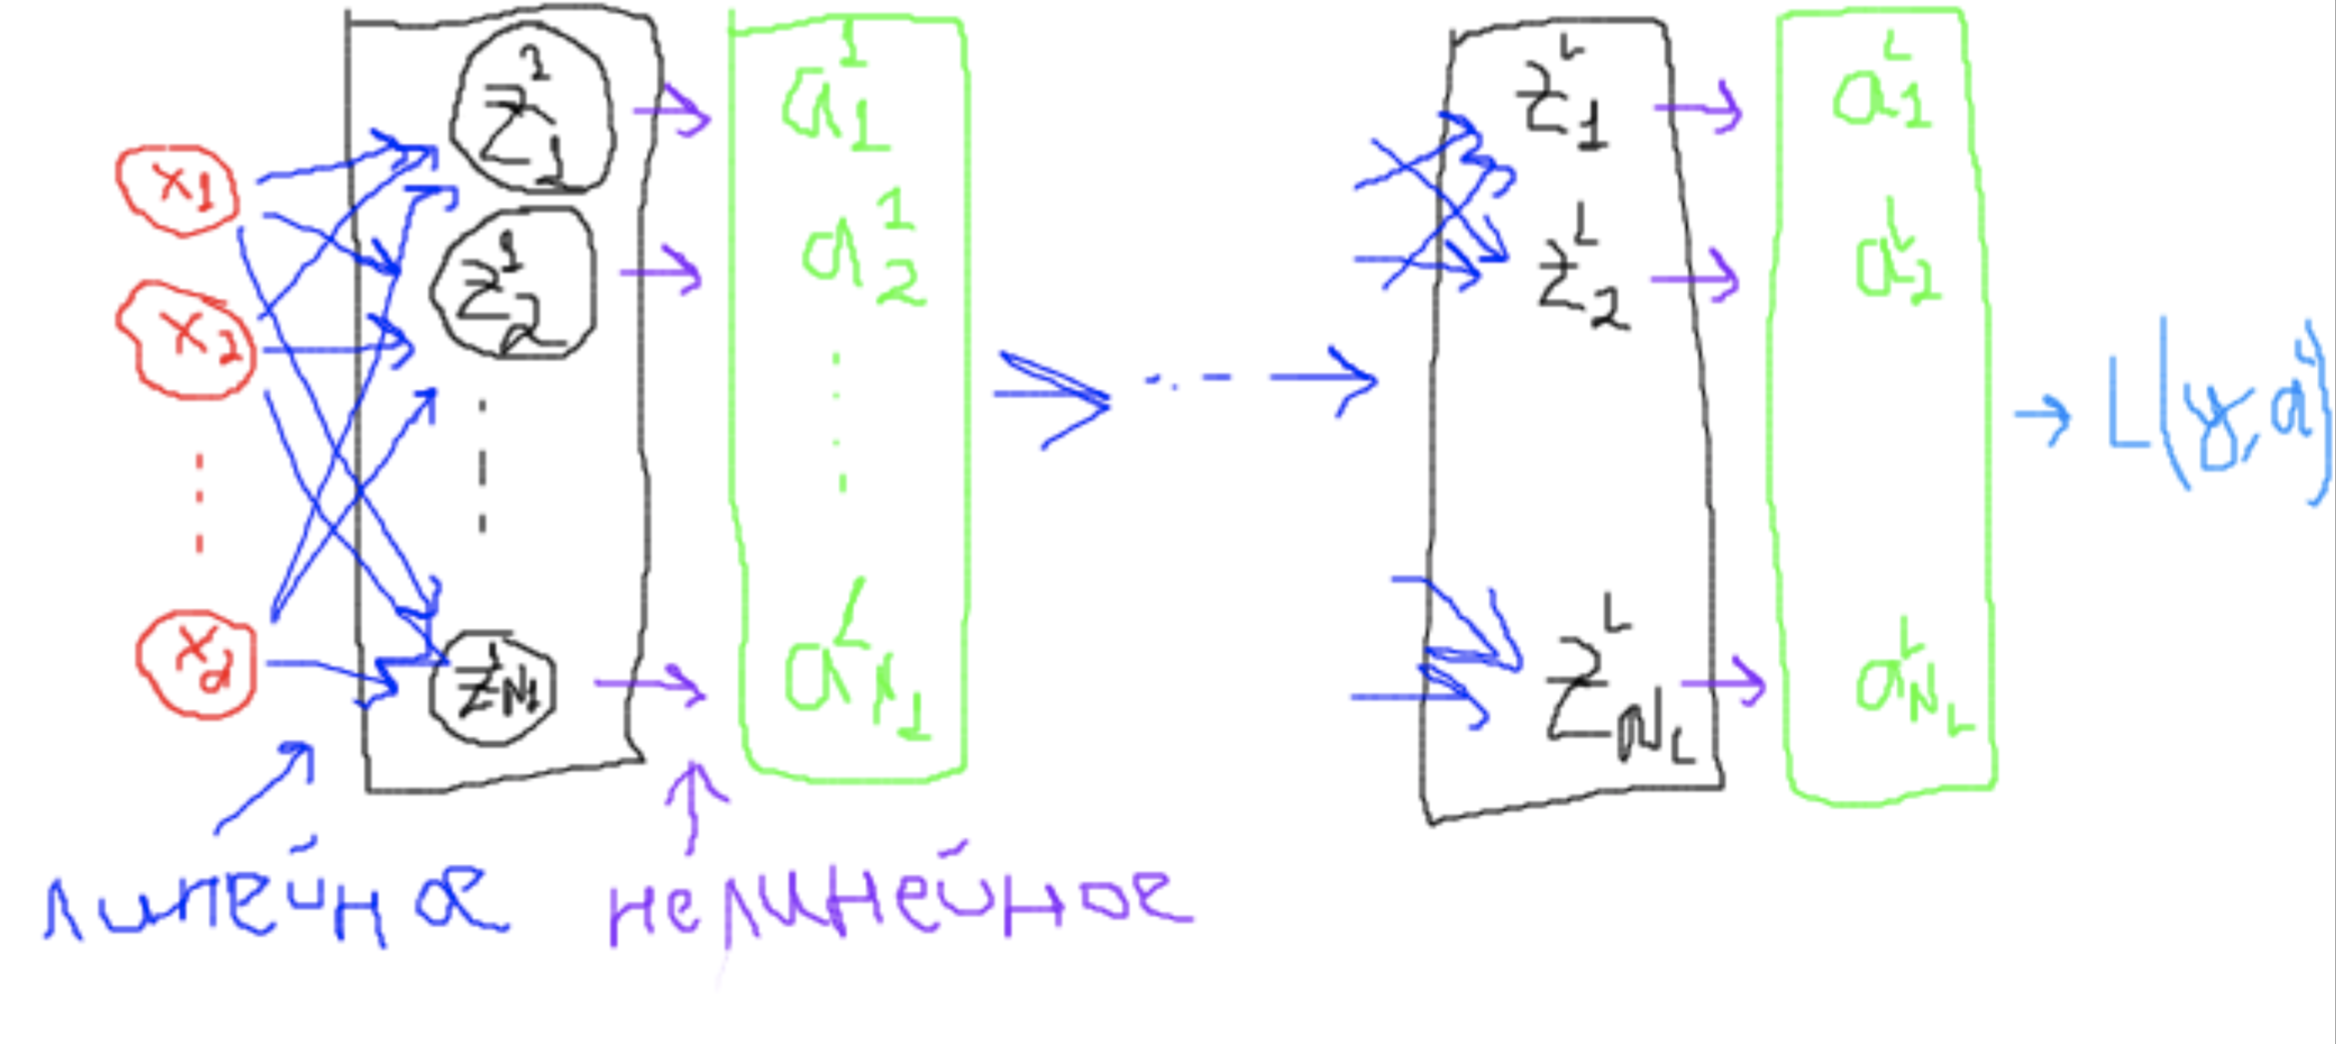
\includegraphics[width=0.9\textwidth]{section/section10_1}}\\
\caption{}
\label{bilet_2_1}
\end{figure}

Пусть у нас задана следующая система преобразований:
$$a_i^0 = x_i \quad z^{l+1} = w_{l+1}^{\mathsf{T}}a^{l} + b_{l+1}, \quad a_{j}^{l+1} = g(z_{j}^{l+1}), \eqno(2.1)$$
где $i \in [1, d]$, $l \in [0, L-1]$, $j \in [1, N_{l+1}]$, $g(t)$ --- некоторая функция активации.

\subsection{функции активации}
\begin{itemize}
	\item $\sigma(z) = \frac{1}{1+\exp(-z)} \in (0,1)$
	\item $\text{tanh} = 2(\sigma(z) - \frac{1}{2}) \in (-1,1)$
	\item $\text{ReLu}(z) = \max(0, z)$
	\item $\text{LeakyRelu}(z) = \max(\alpha z, z), \alpha \in (0,1)$
\end{itemize}

Существует теорема, которая говорит, что любую непрерывную функцию  можно сколь угодно близко приблизить   нейросетью с функцией активации $\sigma(x)$.

\begin{figure}[h!t]\center
\subfloat{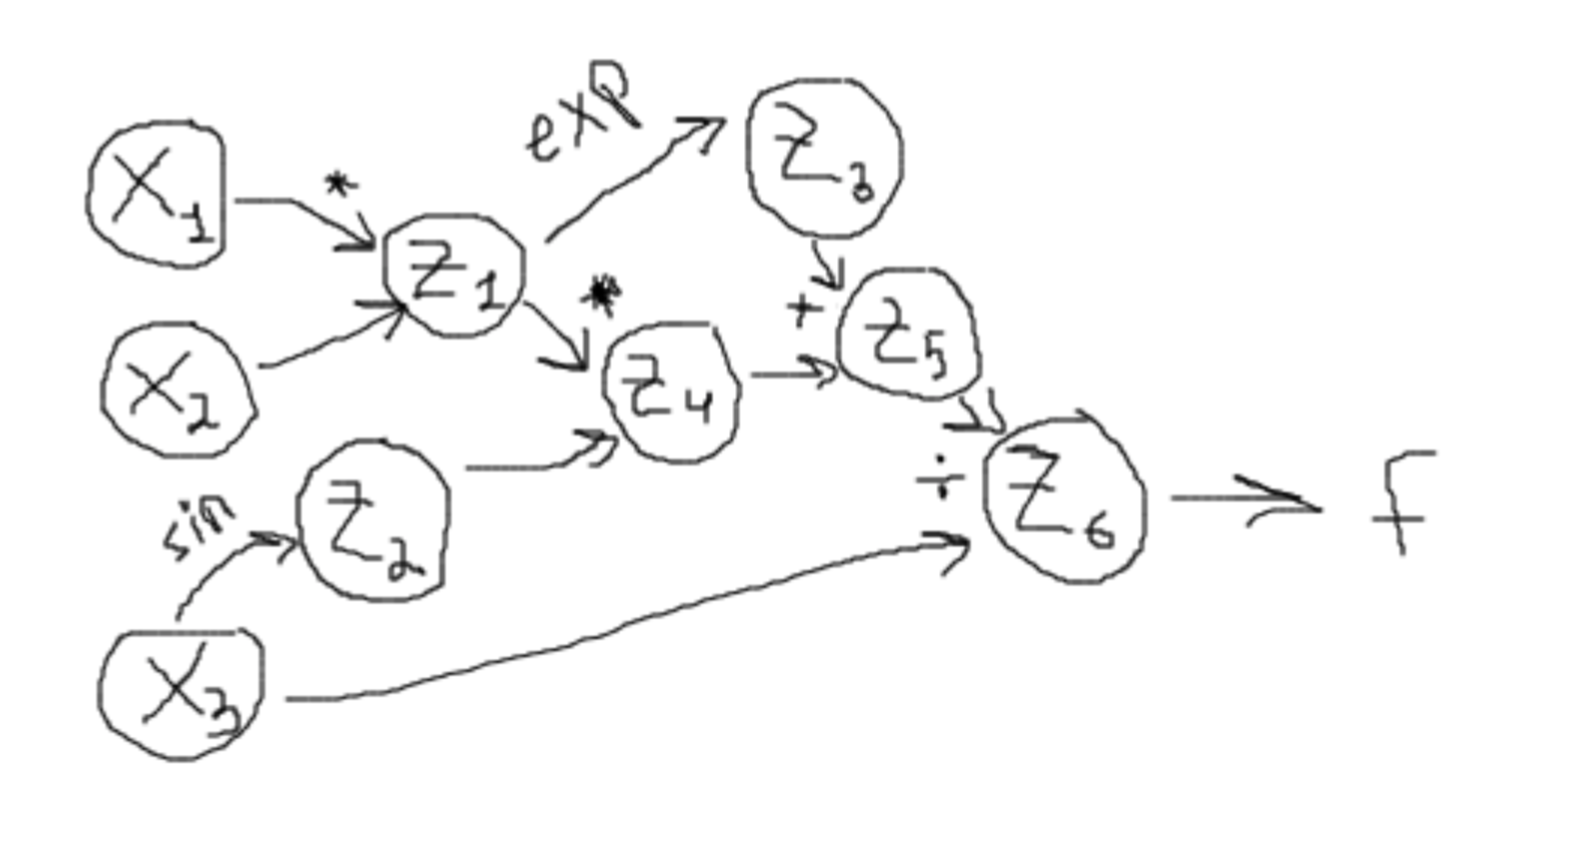
\includegraphics[width=0.9\textwidth]{section/section10_2}}\\
\caption{}
\label{bilet_2_2}
\end{figure}

\subsection{Автоматическое дифференцирование}
Рассмотрим на примере:
$$ f(\textbf{x}) = \frac{x_1x_2\sin(x_3) + \exp(x_1x_2)}{x_3}. \eqno(2.2)$$
Граф вычислений функции (2.2) изображен на рис.~\ref{bilet_2_2}.

Для данной функции посчитаем $\frac{\partial f}{\partial x_1}$ через дифференцирование вперед и дифференцированием назад:\\
~\\
{\bf Дифференцирование вперед:}
\begin{itemize}
	\item $\frac{\partial z_1}{\partial x_1} = x_2$
	\item $\frac{\partial z_2}{\partial x_1} = 0$
	\item $\frac{\partial z_3}{\partial x_1} = \frac{\partial z_3}{\partial z_1}\frac{\partial z_1}{\partial x_1} = \exp(z_1)x_2$
	\item $\frac{\partial z_4}{\partial x_1} = \frac{\partial z_4}{\partial z_1}\frac{\partial z_1}{\partial x_1} + \frac{\partial z_4}{\partial z_2}\frac{\partial z_2}{\partial x_1} = z_2x_2$
	\item $\frac{\partial z_5}{\partial x_1} = \frac{\partial z_5}{\partial z_3}\frac{\partial z_3}{\partial x_1} + \frac{\partial z_5}{\partial z_4}\frac{\partial z_4}{\partial x_1} = \exp(z_1)x_2 + z_2x_2$
	\item $\frac{\partial z_6}{\partial x_1} = \frac{\partial z_6}{\partial x_3}\frac{\partial x_3}{\partial x_1} + \frac{\partial z_6}{\partial z_5}\frac{\partial z_5}{\partial x_1} = \frac{1}{x_3}\left(\exp(z_1)x_2 + z_2x_2\right)$
	\item $\frac{\partial f}{x_1}= \frac{\partial f}{\partial z_6}\frac{\partial z_6}{\partial x_1} = \frac{1}{x_3}\left(\exp(z_1)x_2 + z_2x_2\right)$
\end{itemize}
	~\\

{\bf Дифференцирование назад:}
\begin{itemize}
	\item $\frac{\partial f}{\partial z_6} = 1$
	\item $\frac{\partial f}{\partial z_5} = \frac{\partial f}{\partial z_6}\frac{\partial z_6}{\partial z_5} = \frac{1}{x_3}$
	\item $\frac{\partial f}{\partial z_4} = \frac{\partial f}{\partial z_5}\frac{\partial z_5}{\partial z_4} = \frac{1}{x_3}$
	\item $\frac{\partial f}{\partial z_3} = \frac{\partial f}{\partial z_5}\frac{\partial z_5}{\partial z_3} = \frac{1}{x_3}$
	\item $\frac{\partial f}{\partial z_2} = \frac{\partial f}{\partial z_4}\frac{\partial z_4}{\partial z_2} = \frac{1}{x_3}z_1$
	\item $\frac{\partial f}{\partial z_1} = \frac{\partial f}{\partial z_3}\frac{\partial z_3}{\partial z_1} + \frac{\partial f}{\partial z_4}\frac{\partial z_4}{\partial z_1} = \frac{1}{x_3}\exp(z_1) + \frac{1}{x_3}z_2$
	\item $\frac{\partial f}{\partial x_1} = \frac{\partial f}{\partial z_1}\frac{\partial z_1}{\partial x_1} = \frac{1}{x_3}\left(\exp(z_1) + z_2\right)x_2$
\end{itemize}
	~\\
Как видно результат работы алгоритмов дифференцирования вперед и назад совпадает.
